% ============================================================
% Chapter 17: Problem 16 — Topological Problems in Algebraic Geometry
% ============================================================

\chapter{Topological Problems in Algebraic Geometry}

% ------------------------------------------------------------
\section{Historical Context}
% ------------------------------------------------------------

In the mid-nineteenth century, \textbf{Bernhard Riemann} (1826--1866) transformed mathematics by showing that the study of algebraic curves---the zero sets of polynomial equations in two variables---could be transformed into the study of \emph{topological surfaces}. This insight, one of the significant developments in the history of mathematics, revealed a connection between algebra, geometry, and topology that continues to shape modern mathematics.

\subsection{Riemann Surfaces}

Consider a smooth algebraic curve $C$ defined over the complex numbers, say the curve $y^2 = x^3 - x$ in $\mathbb{C}^2$. At first glance, this is a complicated object: for each complex value of $x$, there are generally two values of $y$ (the square roots of $x^3 - x$), and as $x$ varies over $\mathbb{C}$, the curve ``branches'' at points where $x^3 - x = 0$.

Riemann's approach was to ``unfold'' this multi-valued relationship by replacing $\mathbb{C}^2$ with a new surface---now called a \textbf{Riemann surface}---on which the curve becomes a well-defined, single-valued function. Imagine two copies of the complex plane, slit along certain curves, and glued together in a clever way: the result is a two-dimensional surface on which the algebraic curve lives as a smooth manifold.

\begin{definition}[Riemann surface]
A \textbf{Riemann surface} is a one-dimensional complex manifold---that is, a surface (in the topological sense) equipped with a complex structure at each point, allowing one to perform complex analysis locally. Every smooth algebraic curve over $\mathbb{C}$ gives rise to a compact Riemann surface, and conversely, every compact Riemann surface is algebraic (this deep result is due to Riemann and later formalized by others).
\end{definition}

The Riemann surface corresponding to $y^2 = x^3 - x$ is a \textbf{torus} (a doughnut shape), not a sphere. This is a fact: the topology of the surface---its genus---carries fundamental information about the algebraic curve.

\subsection{The Genus of a Curve}

The \textbf{genus} $g$ of a compact Riemann surface is the number of ``handles'' or ``holes'' it has:
\begin{itemize}
    \item A sphere has genus $g = 0$.
    \item A torus (doughnut) has genus $g = 1$.
    \item A surface with two holes has genus $g = 2$.
\end{itemize}

For a smooth plane curve of degree $d$ in $\mathbb{P}^2$, the genus is given by the famous \textbf{genus formula}:
\[
    g = \frac{(d-1)(d-2)}{2}.
\]
Thus a line ($d=1$) has genus 0, a conic ($d=2$) has genus 0, a cubic ($d=3$) has genus 1, and a quartic ($d=4$) has genus 3. The genus is a \emph{topological invariant}: it does not change under continuous deformations of the surface.

\subsection{The Riemann--Roch Theorem}

Riemann discovered that the genus controls the space of functions on the curve. This insight was made precise by his student Gustav Roch in the \textbf{Riemann--Roch theorem}, one of the fundamental results in algebraic geometry.

\begin{theorem}[Riemann--Roch]\label{thm:riemann-roch}
Let $C$ be a smooth algebraic curve of genus $g$, and let $D$ be a divisor (a formal sum of points on $C$). Then
\[
    \ell(D) - \ell(K - D) = \deg(D) - g + 1
\]
where $\ell(D)$ is the dimension of the space of meromorphic functions $f$ with $(f) + D \geq 0$, $K$ is the canonical divisor (the divisor of a holomorphic 1-form), and $\deg(D)$ is the degree of $D$.
\end{theorem}

For a curve, the canonical divisor $K$ has degree $2g - 2$. When $\deg(D) > 2g - 2$, the term $\ell(K - D)$ vanishes, and the theorem gives an exact formula for $\ell(D)$. The Riemann--Roch theorem shows that the \emph{topology} (the genus) of a curve completely determines many of its algebraic properties---a connection between topology and algebra.

% ------------------------------------------------------------
\begin{figure}[htbp]
\centering
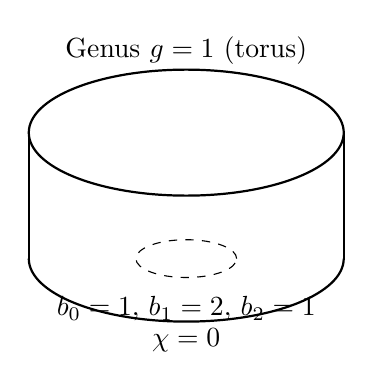
\begin{tikzpicture}[scale=0.8]
  % Draw torus (Riemann surface of genus 1)
  \draw[thick] (0,0) ellipse (2.5 and 1);
  \draw[thick] (-2.5,0) -- (-2.5,-2);
  \draw[thick] (2.5,0) -- (2.5,-2);
  \draw[thick] (-2.5,-2) arc (180:360:2.5 and 1);
  \draw[dashed] (0,-2) ellipse (0.8 and 0.3);
  % Labels
  \node at (0,1.3) {Genus $g = 1$ (torus)};
  \node at (0,-2.8) {$b_0 = 1$, $b_1 = 2$, $b_2 = 1$};
  \node at (0,-3.3) {$\chi = 0$};
\end{tikzpicture}
\caption{A Riemann surface of genus 1 (a torus). The Betti numbers are $b_0 = 1$ (one connected component), $b_1 = 2$ (two independent loops), $b_2 = 1$ (one void). The Euler characteristic is $\chi = 1 - 2 + 1 = 0$.}
\label{fig:riemann-surface-genus-1}
\end{figure}
% ------------------------------------------------------------

\subsection{From Curves to Surfaces: Early Topological Questions}

Riemann's work raised natural questions that went beyond curves:

\begin{itemize}
    \item \textbf{What about surfaces?} An algebraic surface (the zero set of a polynomial in three variables, or a two-dimensional variety) has a much richer topology than a curve. What topological invariants describe a surface? What constraints does the algebraic structure impose?

    \item \textbf{What about higher dimensions?} If algebraic curves give Riemann surfaces, what topology do $n$-dimensional algebraic varieties have? How do the algebraic properties of the variety constrain its topology?

    \item \textbf{How can we compute topological invariants?} Given an algebraic variety defined by equations, how can we compute its Betti numbers, its fundamental group, or its cohomology ring?
\end{itemize}

These questions---roughly speaking---constitute Hilbert's sixteenth problem. Hilbert asked for the development of a general theory connecting algebraic geometry and topology, analogous to what Riemann had achieved for curves.

% ------------------------------------------------------------
\section{The Problem}
% ------------------------------------------------------------

\begin{problem_statement}[Hilbert's Sixteenth Problem]
Hilbert's sixteenth problem has two parts: determine the possible arrangements of the real components of nonsingular algebraic curves (and extend the inquiry to real algebraic surfaces); and find an upper bound, depending on the degree, for the number of limit cycles of a polynomial planar differential equation and study their arrangement.
\end{problem_statement}

The first part belongs to real algebraic geometry and topology; the second is a problem in dynamical systems. Later developments in the topology of complex algebraic varieties are important neighboring subjects, but they are not a substitute for these original questions. The first part includes questions such as:

\begin{enumerate}
    \item \textbf{Topology of real algebraic varieties.} Understand the topology and possible arrangements of the \emph{real} points of algebraic curves and surfaces.
\end{enumerate}

The limit-cycle question asks how many isolated periodic orbits a polynomial vector field of a given degree can have. Both parts remain active, with no general degree-dependent bound known for the limit-cycle problem.

% ------------------------------------------------------------
\section{Key Developments}
% ------------------------------------------------------------

The twentieth century brought powerful tools for studying varieties. The following results provide useful context, although many concern complex varieties and do not directly resolve Hilbert's original real-topology and limit-cycle questions.

\subsection{Related Background: Algebraic Topology}

The early twentieth century saw the birth of \textbf{algebraic topology}, the study of topological spaces through algebraic invariants.

\textbf{Henri Poincar\'e} (1854--1912) introduced the \textbf{fundamental group} of a topological space $X$. It consists of loops based at a point, identified when one can be continuously deformed into the other. For algebraic varieties, the group $\pi_1(X)$ encodes how ``multiply connected'' the space is:
\begin{itemize}
    \item The sphere $\mathbb{S}^2$ is simply connected: $\pi_1(\mathbb{S}^2) = 0$.
    \item The torus $\mathbb{T}^2$ has $\pi_1(\mathbb{T}^2) \cong \mathbb{Z}^2$: there are two independent loops that cannot be contracted.
    \item A Riemann surface of genus $g$ has $\pi_1(\Sigma_g) \cong \langle a_1, b_1, \ldots, a_g, b_g \mid [a_1, b_1] \cdots [a_g, b_g] = 1 \rangle$.
\end{itemize}

\textbf{L.E.J. Brouwer} (1881--1966) introduced \textbf{simplicial homology} and proved foundational results about topological invariance. The \textbf{Betti numbers} $b_k(X) = \rank H_k(X)$ of a topological space count the number of $k$-dimensional ``holes'':
\begin{itemize}
    \item $b_0(X)$ counts connected components.
    \item $b_1(X)$ counts independent loops.
    \item $b_2(X)$ counts independent voids (enclosed cavities).
\end{itemize}

For a smooth complex projective variety of complex dimension $n$ (real dimension $2n$), the Betti numbers satisfy $b_k = b_{2n-k}$ (Poincar\'e duality), and the \textbf{Euler characteristic} $\chi(X) = \sum_{k=0}^{2n} (-1)^k b_k$ is a topological invariant that encodes much information.

\subsection{Sheaf Cohomology: Leray and Serre}

The classical tools of algebraic topology (singular homology, simplicial homology) proved insufficient for the subtle problems of algebraic geometry. A new tool was needed: \textbf{sheaf cohomology}.

\textbf{Jean Leray} (1906--1998), while a prisoner of war in Germany during World War~II, developed the theory of \textbf{spectral sequences} and sheaf cohomology---one of the mathematical achievements of the twentieth century. \textbf{Jean-Pierre Serre} (born 1926) subsequently showed that sheaf cohomology is the right tool for algebraic geometry.

\begin{definition}[Sheaf cohomology]
Let $X$ be a topological space and $\mathcal{F}$ a sheaf of abelian groups on $X$. The \textbf{sheaf cohomology groups} $H^k(X, \mathcal{F})$ are defined as the right derived functors of the global sections functor. They measure the ``failure'' of local cohomological data to patch together globally.
\end{definition}

Serre proved that for a smooth projective variety $X$ over $\mathbb{C}$, the sheaf cohomology groups $H^k(X, \mathbb{Z})$ are \textbf{finitely generated abelian groups} whose ranks are the Betti numbers $b_k$. Moreover, the \textbf{Hodge decomposition} decomposes the complex cohomology:
\[
    H^k(X, \mathbb{C}) = \bigoplus_{p+q=k} H^{p,q}(X)
\]
where $H^{p,q}(X)$ is the space of harmonic $(p,q)$-forms, or equivalently the Dolbeault cohomology group $H^{p,q}_{\bar\partial}(X)$. The dimensions $h^{p,q} = \dim H^{p,q}(X)$ are the \textbf{Hodge numbers}, and they satisfy the symmetry $h^{p,q} = h^{q,p}$ (complex conjugation) and $h^{p,q} = h^{n-p,n-q}$ (Hodge duality). This decomposition is a constraint on the topology of algebraic varieties: not every topological manifold has a Hodge decomposition.

\subsection{The Lefschetz Hyperplane Theorem}

One of the tools for understanding the topology of algebraic varieties is the \textbf{Lefschetz hyperplane theorem}, proved by \textbf{Solomon Lefschetz} (1884--1972) and later generalized by others.

\begin{theorem}[Lefschetz Hyperplane Theorem]\label{thm:lefschetz}
Let $X \subset \mathbb{P}^n$ be a smooth projective variety of dimension $d$, and let $H$ be a smooth hyperplane section (i.e., $H = X \cap \{L = 0\}$ for a general linear form $L$). Then the restriction maps
\[
    H_k(H, \mathbb{Z}) \to H_k(X, \mathbb{Z})
\]
are isomorphisms for $k < d - 1$ and surjective for $k = d - 1$. Dually, the restriction maps
\[
    H^k(X, \mathbb{Z}) \to H^k(H, \mathbb{Z})
\]
are isomorphisms for $k < d - 1$ and injective for $k = d - 1$.
\end{theorem}

In intuitive terms, the theorem says that a hyperplane section of a variety ``sees'' most of the topology of the ambient variety. By slicing repeatedly with hyperplanes, one can reduce questions about the topology of a high-dimensional variety to questions about lower-dimensional sections. This inductive technique is fundamental in algebraic geometry.

\subsection{The Weil Conjectures}

Perhaps the achievement connecting topology and algebraic geometry was the proof of the \textbf{Weil conjectures}, formulated by \textbf{Andr\'e Weil} (1906--1998) in 1949 and proved by \textbf{Alexander Grothendieck} (1928--2014) and \textbf{Pierre Deligne} (born 1944) in 1974.

The Weil conjectures concern the \textbf{zeta function} of a smooth projective variety $X$ over a finite field $\mathbb{F}_q$:
\[
    Z(X, t) = \exp\left(\sum_{n=1}^{\infty} \frac{N_n}{n} t^n\right)
\]
where $N_n = \#X(\mathbb{F}_{q^n})$ is the number of $\mathbb{F}_{q^n}$-rational points of $X$.

\begin{theorem}[Weil Conjectures -- proved]\label{thm:weil-conjectures}
The zeta function $Z(X, t)$ of a smooth projective variety $X$ over $\mathbb{F}_q$ is a \textbf{rational function}:
\[
Z(X, t) = \frac{P_1(t)\cdots P_{2d-1}(t)}{P_0(t)\cdots P_{2d}(t)},
\]
where each $P_i(t)$ is a polynomial with integer coefficients, $P_0(t)=1-t$, $P_{2d}(t)=1-q^d t$. Moreover:
\begin{enumerate}
    \item \textbf{Rationality:} $Z(X, t)$ is a rational function.
    \item \textbf{Functional equation:} $Z\!\left(X,\frac{1}{q^d t}\right)=\pm q^{d\chi/2}t^{\chi}Z(X,t)$, where $\chi=\chi(X)$ is the Euler characteristic.
    \item \textbf{Riemann hypothesis:} The reciprocal roots of $P_i(t)$ have absolute value $q^{i/2}$ (equivalently, the roots of $P_i$ have absolute value $q^{-i/2}$).
    \item \textbf{Cohomological interpretation:} $P_i(t)$ is the characteristic polynomial of Frobenius on $i$th $\ell$-adic cohomology, and its degree is the corresponding Betti number.
\end{enumerate}
\end{theorem}

The Weil conjectures are notable because they connect:
\begin{itemize}
    \item \textbf{Algebra} (counting solutions over finite fields),
    \item \textbf{Topology} (Betti numbers and Euler characteristic),
    \item \textbf{Number theory} (the distribution of rational points).
\end{itemize}

Grothendieck's contribution was to reformulate the conjectures in terms of \textbf{\'{e}tale cohomology}, a new cohomology theory for algebraic varieties defined over arbitrary fields (not just $\mathbb{C}$). The key insight was that \'etale cohomology should behave like singular cohomology but work over finite fields. Grothendieck proved rationality and the functional equation. Deligne completed the proof by establishing the deepest part---the Riemann hypothesis---using an argument involving estimates for l-adic sheaves.

The Weil conjectures demonstrate that the topology of an algebraic variety (encoded in its Betti numbers and cohomology) controls its arithmetic behavior (the number of rational points). This is a vindication of Hilbert's intuition that topology and algebraic geometry are intertwined.

\subsection{Neighboring Open Problem: The Hodge Conjecture}

The \textbf{Hodge conjecture} is a major open problem in algebraic geometry and one of the seven \textbf{Clay Millennium Problems}. It is related to the broad interaction between topology and algebraic geometry, but it is not one of the two questions Hilbert posed in his sixteenth problem.

\begin{conjecture}[Hodge Conjecture]\label{conj:hodge}
Let $X$ be a smooth complex projective variety of dimension $n$. Then every \textbf{Hodge class}---every element of $H^{2k}(X, \mathbb{Q}) \cap H^{k,k}(X)$---is a rational linear combination of classes of algebraic subvarieties of codimension~$k$.
\end{conjecture}

In other words, certain topological cycles on algebraic varieties (those satisfying a condition from the Hodge decomposition) must be ``algebraic'': they must come from actual algebraic subvarieties. This would mean that the Hodge decomposition---a priori a topological or analytic invariant---completely detects algebraic subvarieties.

\begin{itemize}
    \item The Hodge conjecture is \textbf{trivially true} in dimension 1: every class in $H^{1,1}$ on a curve is algebraic.
    \item For surfaces (dimension 2), the Hodge conjecture is known for classes in $H^{1,1}$ (the Lefschetz $(1,1)$-theorem, proved by Lefschetz and later generalized): every integral $(1,1)$-class on a surface is the class of a divisor.
    \item For higher codimension, the Hodge conjecture remains \textbf{wide open} in general. It is known in special cases (e.g., for abelian varieties of small dimension, and for some specific classes), but no general proof is known.
\end{itemize}

The Hodge conjecture connects the \emph{analytic} structure of a variety (the Hodge decomposition) to its \emph{algebraic} structure (the existence of algebraic subvarieties). If true, it would establish a perfect correspondence between topology and algebra for complex projective varieties.

\subsection{The Topology of Real Algebraic Varieties}

Hilbert also asked about the topology of \textbf{real algebraic varieties}---the sets of real solutions to polynomial equations. This aspect of the problem is closely related to \textbf{real algebraic geometry} and \textbf{real enumerative geometry}.

Key results include:

\begin{itemize}
    \item \textbf{Harnack's theorem} (1876): A smooth real projective curve of degree $d$ has at most $g + 1$ connected components (ovals), where $g = (d-1)(d-2)/2$ is the genus. Moreover, this bound is achieved for curves of every degree.

    \item \textbf{The Smith--Thom inequality}: For a smooth projective variety defined over $\mathbb{R}$, the sum of the Betti numbers of $X(\mathbb{R})$ with $\mathbb{Z}/2\mathbb{Z}$ coefficients is at most the corresponding sum for $X(\mathbb{C})$. This is an inequality for total Betti numbers, not Euler characteristics.

    \item \textbf{Viro's patchworking method}: A powerful technique for constructing real algebraic varieties with prescribed topology, connecting tropical geometry to real algebraic geometry.

    \item \textbf{Thom's conjecture} (and its generalizations): The topology of real algebraic surfaces in $\mathbb{R}^3$ is highly constrained. For instance, the maximal number of connected components of a smooth real algebraic surface of degree $d$ in $\mathbb{R}^3$ is an active area of research.
\end{itemize}

These results are relevant background, but Hilbert's first part asks specifically about possible real topological types and arrangements, while the second part concerns limit cycles.

\subsection{Limit Cycles of Polynomial Vector Fields}

A \textbf{limit cycle} is an isolated periodic orbit of a planar differential equation. Hilbert's second question asks for a uniform upper bound on the number of limit cycles of a polynomial vector field of degree $d$, and for a description of their possible configurations. Methods from dynamical systems and algebraic geometry settle special low-degree cases, but no general bound as a function of $d$ is known. This is the central open part of Hilbert's sixteenth problem.

% ------------------------------------------------------------
\section{Current Status: Partially Solved}
% ------------------------------------------------------------

\begin{partiallybox}
Hilbert's sixteenth problem remains open in substantial part. Harnack's theorem gives the maximum number of components of a nonsingular real plane curve, and many arrangements have been classified in low degrees; higher-degree classification and the topology of real algebraic surfaces are not fully settled. No general upper bound is known for the number of limit cycles of a polynomial planar vector field in terms of its degree. The Hodge conjecture and the Weil conjectures discussed above are important neighboring topics, not solutions to either part of Hilbert's problem.
\end{partiallybox}

% ------------------------------------------------------------
\section*{Common Questions}

\begin{description}[font=\bfseries, leftmargin=2em, style=nextline]

\item[Q: What's the difference between an algebraic variety and a manifold?]\hfill\\
A manifold is a space that locally looks like $\mathbb{R}^n$ (smooth and without singularities). An algebraic variety is the zero set of a system of polynomial equations, and it can have \emph{singularities}---points where it is not smooth, like the tip of a cone ($x^2 + y^2 = z^2$). Over the complex numbers, a smooth algebraic variety is a complex manifold, but not all complex manifolds are algebraic. The interplay between these two viewpoints---algebraic equations and smooth topology---is at the heart of Hilbert's 16th problem.

\item[Q: What are the Weil conjectures in simple terms?]\hfill\\
The Weil conjectures (proved by Deligne in 1974) relate the number of solutions to polynomial equations over finite fields to the topological structure of the corresponding complex algebraic variety. They predicted that the generating function counting solutions modulo $p$, modulo $p^2$, etc. is a rational function whose properties mirror the topology (Betti numbers, Poincaré duality) of the variety over $\mathbb{C}$. This is notable: counting points over finite fields reveals the shape of a space over the complex numbers.

\item[Q: What's the Hodge conjecture about?]\hfill\\
The Hodge conjecture asks whether every rational cohomology class of Hodge type $(p,p)$ on a smooth complex projective variety is a rational linear combination of classes of algebraic cycles. It is one of the Clay Millennium Problems and remains open.

\item[Q: Why are real algebraic varieties harder than complex ones?]\hfill\\
Over $\mathbb{C}$, the fundamental theorem of algebra guarantees that polynomial equations always have solutions, and the topology is governed by powerful tools like sheaf cohomology and Hodge theory. Over $\mathbb{R}$, a polynomial equation can have no real solutions at all, components can appear and disappear as parameters change, and the topology (number of ovals, their nesting, etc.) is much more delicate. Hilbert's 16th problem specifically asks about the topology of \emph{real} algebraic curves and surfaces, which remains only partially understood.

\item[Q: What is a Lefschetz pencil?]\hfill\\
A Lefschetz pencil is a family of hyperplane sections of a projective variety, parameterized by a line in the dual projective space. It is a central tool for studying topology: as the hyperplane varies, the sections change smoothly except at finitely many singular fibers, typically acquiring a node. The associated vanishing cycles describe how the homology changes; under the usual hypotheses they generate the kernel of the map from a smooth fiber's middle homology to the ambient variety's homology. Lefschetz's work established a powerful connection between equations and topology.

\item[Q: How does Hilbert's 16th problem split into two parts?]\hfill\\
The first part asks about the possible arrangements of components of real algebraic curves and the topology of real algebraic surfaces. Harnack's theorem gives the maximum number of components of a nonsingular plane curve, while the classification of arrangements is complete only in limited ranges. The second part asks for bounds on the number and arrangement of limit cycles of polynomial planar vector fields; no general bound in terms of the degree is known.

\end{description}

% ------------------------------------------------------------
\section*{Key Takeaways}

\begin{enumerate}
    \item Hilbert's sixteenth problem has two parts: arrangements of real algebraic curves and surfaces, and the number and arrangement of limit cycles of polynomial planar systems.
    \item The Riemann--Roch theorem relates the geometry of a curve to its topology.
    \item Hodge theory connects topology to complex geometry via harmonic forms.
    \item The Weil conjectures (proved by Deligne) connect topology to number theory.
    \item The Hodge conjecture, one of the Clay Millennium Problems, remains open.
\end{enumerate}

\section*{Exercises}
% ------------------------------------------------------------

\begin{enumerate}

    \item \textbf{Genus of plane curves.}
    \begin{enumerate}
        \item Compute the genus of a smooth plane curve of degree $d = 4$ (a quartic) using the formula $g = (d-1)(d-2)/2$.
        \item What is the genus of a smooth plane curve of degree $d = 5$ (a quintic)?
        \item A smooth plane cubic ($d = 3$) has genus 1. Its Riemann surface is a torus. Explain why this means that a cubic curve has a group structure (the sum of two points on the curve can be defined geometrically using lines through the curve).
    \end{enumerate}

    \item \textbf{Betti numbers of surfaces.}
    \begin{enumerate}
        \item The sphere $\mathbb{S}^2$ has Betti numbers $b_0 = 1$, $b_1 = 0$, $b_2 = 1$. Compute the Euler characteristic $\chi(\mathbb{S}^2) = b_0 - b_1 + b_2$.
        \item A torus $\mathbb{T}^2$ has Betti numbers $b_0 = 1$, $b_1 = 2$, $b_2 = 1$. Compute $\chi(\mathbb{T}^2)$.
        \item A Riemann surface of genus $g$ has Betti numbers $b_0 = 1$, $b_1 = 2g$, $b_2 = 1$. Show that $\chi = 2 - 2g$. Verify this for $g = 0$ (sphere) and $g = 1$ (torus).
        \item A smooth curve of degree 4 in $\mathbb{P}^2$ has genus 3. What is its Euler characteristic?
    \end{enumerate}

    \item \textbf{Fundamental groups.}
    \begin{enumerate}
        \item The fundamental group of the sphere $\mathbb{S}^2$ is trivial: $\pi_1(\mathbb{S}^2) = 0$. Explain what this means intuitively (every loop on the sphere can be contracted to a point).
        \item The fundamental group of the torus $\mathbb{T}^2$ is $\mathbb{Z} \times \mathbb{Z}$. Describe two loops on the torus that generate this group.
        \item The fundamental group of a Riemann surface of genus $g \geq 1$ is the surface group $\langle a_1, b_1, \ldots, a_g, b_g \mid [a_1, b_1] \cdots [a_g, b_g] = 1 \rangle$. For $g = 1$, this reduces to $\langle a, b \mid aba^{-1}b^{-1} = 1 \rangle \cong \mathbb{Z}^2$, consistent with the torus.
    \end{enumerate}

    \item \textbf{The Hodge diamond.}
    \begin{enumerate}
        \item The Hodge numbers $h^{p,q} = \dim H^{p,q}(X)$ of a smooth complex projective variety are arranged in a diamond-shaped array called the \textbf{Hodge diamond}. For a smooth curve of genus $g$, the Hodge diamond is:
        \[
        \begin{array}{ccc}
         & h^{0,0} & \\
        h^{1,0} & & h^{0,1} \\
         & h^{1,1} &
        \end{array}
        = 
        \begin{array}{ccc}
         & 1 & \\
        g & & g \\
         & 1 &
        \end{array}
        \]
        Verify that $h^{p,q}$ satisfies $h^{p,q} = h^{q,p}$ (symmetry) and that $\sum_{p+q=k} h^{p,q} = b_k$ (the $k$-th Betti number).
        \item For a smooth projective surface $S$, the Hodge numbers satisfy $h^{0,0} = h^{2,2} = 1$, $h^{1,0} = h^{0,1} = h^{2,1} = h^{1,2}$, $h^{2,0} = h^{0,2}$, and $h^{1,1}$ is determined by the Euler characteristic. If $S$ is a smooth quartic surface in $\mathbb{P}^3$, show that $\chi(S) = 24$ and compute the Hodge numbers.
    \end{enumerate}

    \item \textbf{Lefschetz hyperplane theorem (intuition).}
    \begin{enumerate}
        \item Let $C$ be a smooth plane curve of degree $d$ in $\mathbb{P}^2$ (so $C$ has complex dimension 1, real dimension 2). The Lefschetz hyperplane theorem says that the map $H_0(C) \to H_0(\mathbb{P}^2)$ is an isomorphism (both spaces are connected) and $H_1(C) \to H_1(\mathbb{P}^2)$ is surjective. Since $H_1(\mathbb{P}^2) = 0$, this says $H_1(C)$ surjects onto 0---which is trivially true. The interesting content is that $H^1(C)$ carries information about $C$ that is \emph{new}: it is not detected by the ambient $\mathbb{P}^2$. Explain why this is consistent with the fact that $b_1(C) = 2g > 0$ for $g \geq 1$.
        \item For a smooth surface $S$ in $\mathbb{P}^3$, the Lefschetz theorem says $H_1(S) \cong H_1(\mathbb{P}^3) = 0$ and $H_2(S)$ surjects onto $H_2(\mathbb{P}^3) \cong \mathbb{Z}$. What does this tell you about $b_1(S)$?
    \end{enumerate}

    \item[$\star$] \textbf{The Weil conjectures and point counting.}
    \begin{enumerate}
        \item Let $X = \mathbb{P}^1$ (the projective line) over $\mathbb{F}_q$. The zeta function is $Z(\mathbb{P}^1, t) = 1 / ((1-t)(1-qt))$. Compute $N_n = \#X(\mathbb{F}_{q^n})$ from this zeta function and verify that $N_n = q^n + 1$. (This counts the points of $\mathbb{P}^1(\mathbb{F}_{q^n})$: the $q^n$ affine points plus the point at infinity.)
        \item The Betti numbers of $\mathbb{P}^1 \cong \mathbb{S}^2$ are $b_0 = 1$, $b_1 = 0$, $b_2 = 1$. The Euler characteristic is $\chi = 2$. Verify that the functional equation of the zeta function holds for $\mathbb{P}^1$.
        \item (Optional) Compute the zeta function of the elliptic curve $E: y^2 = x^3 + x$ over $\mathbb{F}_3$. Count the points $N_1 = \#E(\mathbb{F}_3)$ and $N_2 = \#E(\mathbb{F}_9)$, and verify that $Z(E, t) = (1 - at + 3t^2) / ((1-t)(1-3t))$ where $a = 3 + 1 - N_1$.
    \end{enumerate}

    \item[$\star$] \textbf{Real algebraic curves (Harnack's theorem).}
    \begin{enumerate}
        \item A smooth real conic ($d = 2$) has genus 0, so it has at most $0 + 1 = 1$ connected component. Verify: the conic $x^2 + y^2 = 1$ in $\mathbb{R}^2$ (one component) and $x^2 + y^2 = -1$ (empty, zero components) are the only possibilities. (In $\mathbb{P}^2(\mathbb{R})$, the conic $x^2 + y^2 = z^2$ is one component; $x^2 + y^2 = -z^2$ is empty.)
        \item A smooth real cubic ($d = 3$) has genus 1, so it has at most 2 connected components. The cubic $y^2 = x^3 - x$ has two components: an oval and an unbounded branch. Verify this by plotting the curve. The cubic $y^2 = x^3 + x$ has only one component (no oval). Explain why this is consistent with Harnack's bound.
        \item A smooth real quartic ($d = 4$) has genus 3, so it has at most 4 connected components. Can you find a real quartic with 4 components? (Hint: try $(x^2 + y^2 - 1)(x^2 + y^2 - 4) = 0$---but this is singular. A smooth quartic with 4 ovals is known as a \textbf{M-curve}.)
    \end{enumerate}

\end{enumerate}
